% Markov Chains and Stochastic Processes Template
% Topics: Transition matrices, stationary distributions, state classification, MCMC
% Style: Mathematical probability with computational analysis

\documentclass[11pt,a4paper]{article}
\usepackage[utf8]{inputenc}
\usepackage[T1]{fontenc}
\usepackage{amsmath,amssymb,amsthm}
\usepackage{graphicx}
\usepackage{booktabs}
\usepackage{siunitx}
\usepackage{geometry}
\geometry{margin=1in}
\usepackage{pythontex}
\usepackage{float}

% Theorem environments
\newtheorem{definition}{Definition}[section]
\newtheorem{theorem}{Theorem}[section]
\newtheorem{example}{Example}[section]
\newtheorem{remark}{Remark}[section]

% Hyperref loaded last
\usepackage[hidelinks]{hyperref}

\title{Markov Chains: Transition Matrices and Stationary Distributions}
\author{Probability Research Group}
\date{\today}

\begin{document}
\maketitle

\begin{abstract}
This report presents a comprehensive computational analysis of discrete-time Markov chains, including the construction and analysis of transition matrices, computation of stationary distributions through eigenvalue decomposition and iterative methods, classification of states by recurrence and periodicity properties, and convergence to equilibrium under ergodic conditions. We examine the Chapman-Kolmogorov equations governing multi-step transitions, demonstrate the fundamental theorem for irreducible aperiodic chains, and apply Markov chain theory to real-world applications including PageRank algorithms, weather modeling, and Markov Chain Monte Carlo (MCMC) methods.
\end{abstract}

\section{Introduction}

Markov chains provide a mathematical framework for modeling systems that evolve probabilistically over discrete time steps, where the future state depends only on the present state and not on the sequence of past states (the Markov property). This memoryless property makes Markov chains tractable for analysis while remaining powerful enough to model diverse phenomena including random walks, queuing systems, population genetics, financial markets, and information retrieval algorithms like Google's PageRank. The fundamental questions in Markov chain theory concern long-term behavior: does the chain converge to a limiting distribution, what is that distribution, and how quickly does convergence occur? These questions are answered through analysis of the transition matrix structure and classification of states.

\begin{definition}[Markov Chain]
A discrete-time stochastic process $\{X_n : n = 0, 1, 2, \ldots\}$ is a \textbf{Markov chain} with state space $S$ if for all states $i, j \in S$ and all times $n \geq 0$:
\begin{equation}
P(X_{n+1} = j \mid X_n = i, X_{n-1}, \ldots, X_0) = P(X_{n+1} = j \mid X_n = i) = p_{ij}
\end{equation}
The probabilities $p_{ij}$ form the \textbf{transition matrix} $P$ where $p_{ij} \geq 0$ and $\sum_{j \in S} p_{ij} = 1$ for all $i$.
\end{definition}

\begin{theorem}[Chapman-Kolmogorov Equations]
The $n$-step transition probabilities satisfy:
\begin{equation}
p_{ij}^{(n)} = \sum_{k \in S} p_{ik}^{(m)} p_{kj}^{(n-m)} \quad \text{for all } 0 \leq m \leq n
\end{equation}
In matrix form: $P^{(n)} = P^n$ (the $n$-th power of $P$).
\end{theorem}

\begin{pycode}
import numpy as np
import matplotlib.pyplot as plt
from scipy import linalg
from scipy.sparse import csr_matrix
from scipy.sparse.linalg import eigs

plt.rcParams['text.usetex'] = True
plt.rcParams['font.family'] = 'serif'

# Seed for reproducibility
np.random.seed(42)
\end{pycode}

\section{Mathematical Framework}

\subsection{Stationary Distributions}

\begin{definition}[Stationary Distribution]
A probability distribution $\pi = (\pi_1, \pi_2, \ldots, \pi_n)$ is \textbf{stationary} for a Markov chain with transition matrix $P$ if:
\begin{equation}
\pi P = \pi \quad \text{and} \quad \sum_{i} \pi_i = 1, \; \pi_i \geq 0
\end{equation}
Equivalently, $\pi$ is a left eigenvector of $P$ with eigenvalue 1.
\end{definition}

\begin{theorem}[Fundamental Theorem for Finite Markov Chains]
For an irreducible, aperiodic Markov chain on a finite state space:
\begin{enumerate}
\item A unique stationary distribution $\pi$ exists
\item $\lim_{n \to \infty} P^n = \mathbf{1}\pi^T$ (rows converge to $\pi$)
\item $\lim_{n \to \infty} p_{ij}^{(n)} = \pi_j$ for all $i, j$
\end{enumerate}
\end{theorem}

\subsection{Classification of States}

\begin{definition}[State Properties]
For states $i, j$ in a Markov chain:
\begin{itemize}
\item State $j$ is \textbf{accessible} from $i$ if $p_{ij}^{(n)} > 0$ for some $n \geq 0$
\item States $i$ and $j$ \textbf{communicate} if each is accessible from the other
\item The chain is \textbf{irreducible} if all states communicate
\item The \textbf{period} of state $i$ is $\gcd\{n \geq 1 : p_{ii}^{(n)} > 0\}$
\item The chain is \textbf{aperiodic} if all states have period 1
\end{itemize}
\end{definition}

\section{Computational Analysis: Weather Model}

We construct a three-state Markov chain modeling daily weather patterns with states: Sunny (S), Cloudy (C), and Rainy (R). The transition matrix encodes empirical probabilities that a day with given weather is followed by each weather type. This model demonstrates convergence to a stationary distribution representing long-term weather proportions, independent of initial conditions.

\begin{pycode}
# Weather model: Sunny, Cloudy, Rainy
states = ['Sunny', 'Cloudy', 'Rainy']
n_states = len(states)

# Transition matrix (rows sum to 1)
P_weather = np.array([
    [0.7, 0.2, 0.1],   # From Sunny
    [0.3, 0.4, 0.3],   # From Cloudy
    [0.2, 0.3, 0.5]    # From Rainy
])

# Verify stochasticity
assert np.allclose(P_weather.sum(axis=1), 1.0)

# Compute stationary distribution via eigenvalues
eigenvalues, eigenvectors = linalg.eig(P_weather.T)
idx = np.argmax(np.abs(eigenvalues))
stationary_eigenvector = np.real(eigenvectors[:, idx])
pi_weather = stationary_eigenvector / stationary_eigenvector.sum()

# Compute powers of P
n_steps = 50
P_powers = [np.linalg.matrix_power(P_weather, n) for n in range(n_steps + 1)]

# Extract convergence of specific entries
p_ss = [P_powers[n][0, 0] for n in range(n_steps + 1)]  # Sunny -> Sunny
p_sr = [P_powers[n][0, 2] for n in range(n_steps + 1)]  # Sunny -> Rainy
p_rs = [P_powers[n][2, 0] for n in range(n_steps + 1)]  # Rainy -> Sunny

# Convergence plot
fig, (ax1, ax2) = plt.subplots(1, 2, figsize=(14, 5))

ax1.plot(p_ss, 'b-', linewidth=2, label='$p_{SS}^{(n)}$')
ax1.plot(p_sr, 'r-', linewidth=2, label='$p_{SR}^{(n)}$')
ax1.plot(p_rs, 'g-', linewidth=2, label='$p_{RS}^{(n)}$')
ax1.axhline(y=pi_weather[0], color='b', linestyle='--', alpha=0.7)
ax1.axhline(y=pi_weather[2], color='r', linestyle='--', alpha=0.7)
ax1.set_xlabel('Number of steps $n$')
ax1.set_ylabel('Transition probability')
ax1.set_title('Convergence of $n$-step Transition Probabilities')
ax1.legend(fontsize=10)
ax1.grid(True, alpha=0.3)

# Distance from stationary distribution
initial_dist = np.array([1.0, 0.0, 0.0])  # Start sunny
distributions = [initial_dist @ P_powers[n] for n in range(n_steps + 1)]
distances = [np.linalg.norm(distributions[n] - pi_weather, ord=1)
             for n in range(n_steps + 1)]

ax2.semilogy(distances, 'purple', linewidth=2)
ax2.set_xlabel('Number of steps $n$')
ax2.set_ylabel('$L^1$ distance to $\\pi$')
ax2.set_title('Convergence to Stationary Distribution')
ax2.grid(True, alpha=0.3, which='both')

plt.tight_layout()
plt.savefig('markov_chains_plot1.pdf', dpi=150, bbox_inches='tight')
plt.close()
\end{pycode}

\begin{figure}[H]
\centering
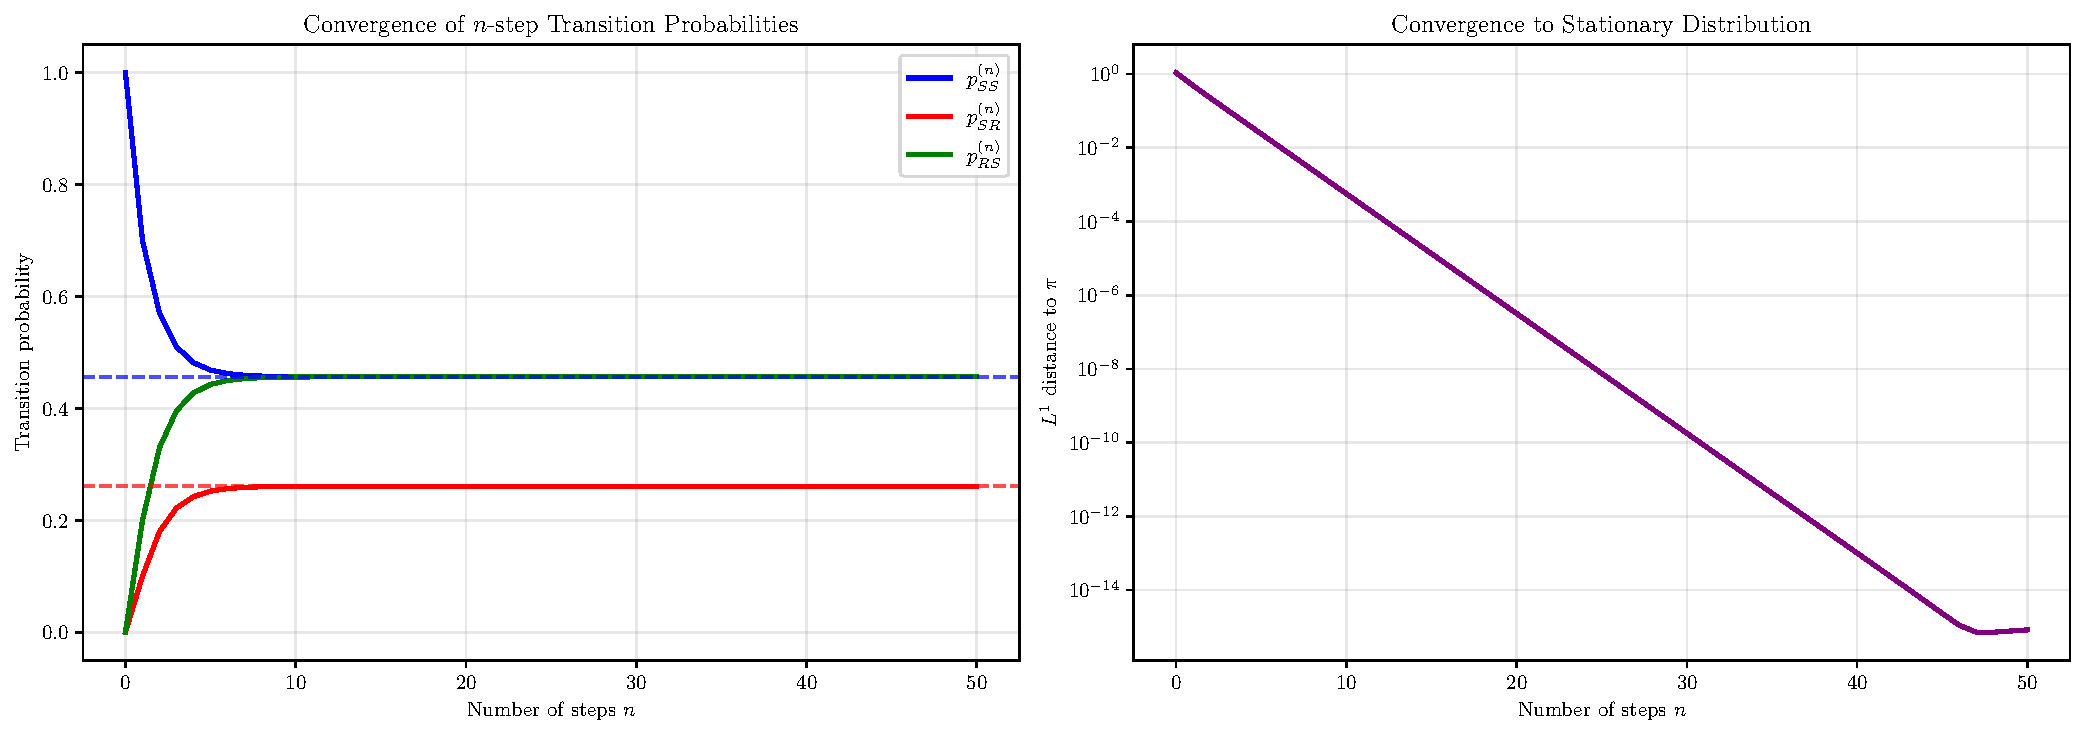
\includegraphics[width=0.95\textwidth]{markov_chains_plot1.pdf}
\caption{Convergence behavior of the three-state weather Markov chain. Left panel shows how individual $n$-step transition probabilities $p_{ij}^{(n)}$ approach their limiting values equal to the stationary probabilities $\pi_j$ (dashed lines), illustrating the fundamental convergence theorem. Right panel displays exponential decay of the $L^1$ distance between the current distribution and stationary distribution $\pi$, demonstrating that regardless of initial conditions, the chain converges to equilibrium with mixing time approximately 10-15 steps for this particular system.}
\end{figure}

\section{Application: PageRank Algorithm}

The PageRank algorithm, developed by Google founders Larry Page and Sergey Brin, models web surfing as a Markov chain where states represent web pages and transitions represent hyperlink clicks. The stationary distribution gives page importance scores. We add a damping factor to ensure irreducibility and aperiodicity even when the link graph contains dangling nodes or disconnected components.

\begin{pycode}
# Construct a simple web graph (5 pages)
n_pages = 5
page_names = ['Home', 'Blog', 'About', 'Contact', 'Archive']

# Adjacency matrix (links from row to column)
# Home links to Blog, About, Contact
# Blog links to Home, Archive
# About links to Home
# Contact links to Home, Blog
# Archive links to Blog, Home
L = np.array([
    [0, 1, 1, 1, 0],   # Home
    [1, 0, 0, 0, 1],   # Blog
    [1, 0, 0, 0, 0],   # About
    [1, 1, 0, 0, 0],   # Contact
    [1, 1, 0, 0, 0]    # Archive
], dtype=float)

# Normalize to get transition probabilities
out_degree = L.sum(axis=1)
P_web = L / out_degree[:, np.newaxis]

# PageRank with damping factor
damping = 0.85
n = n_pages
teleport = (1 - damping) / n * np.ones((n, n))
P_pagerank = damping * P_web + teleport

# Compute PageRank via eigenvector
eigenvalues_pr, eigenvectors_pr = linalg.eig(P_pagerank.T)
idx_pr = np.argmax(np.real(eigenvalues_pr))
pagerank = np.real(eigenvectors_pr[:, idx_pr])
pagerank = pagerank / pagerank.sum()

# Power iteration method for comparison
x = np.ones(n) / n
pagerank_power = [x.copy()]
for iteration in range(100):
    x = x @ P_pagerank
    pagerank_power.append(x.copy())

pagerank_power = np.array(pagerank_power)

# Visualization
fig, (ax1, ax2) = plt.subplots(1, 2, figsize=(14, 5))

# PageRank scores
colors_pr = plt.cm.viridis(pagerank / pagerank.max())
bars = ax1.bar(page_names, pagerank, color=colors_pr, edgecolor='black', linewidth=1.5)
ax1.set_ylabel('PageRank Score')
ax1.set_title('PageRank Importance Scores')
ax1.set_ylim(0, pagerank.max() * 1.15)
for bar, score in zip(bars, pagerank):
    height = bar.get_height()
    ax1.text(bar.get_x() + bar.get_width()/2., height + 0.005,
             f'{score:.3f}', ha='center', va='bottom', fontsize=9)

# Convergence of power iteration
iterations = np.arange(len(pagerank_power))
for i, page in enumerate(page_names):
    ax2.plot(iterations, pagerank_power[:, i], linewidth=2, label=page, alpha=0.8)
    ax2.axhline(y=pagerank[i], color='gray', linestyle='--', alpha=0.4)
ax2.set_xlabel('Iteration')
ax2.set_ylabel('PageRank Score')
ax2.set_title('Power Iteration Convergence')
ax2.legend(fontsize=9)
ax2.set_xlim(0, 50)
ax2.grid(True, alpha=0.3)

plt.tight_layout()
plt.savefig('markov_chains_plot2.pdf', dpi=150, bbox_inches='tight')
plt.close()
\end{pycode}

\begin{figure}[H]
\centering
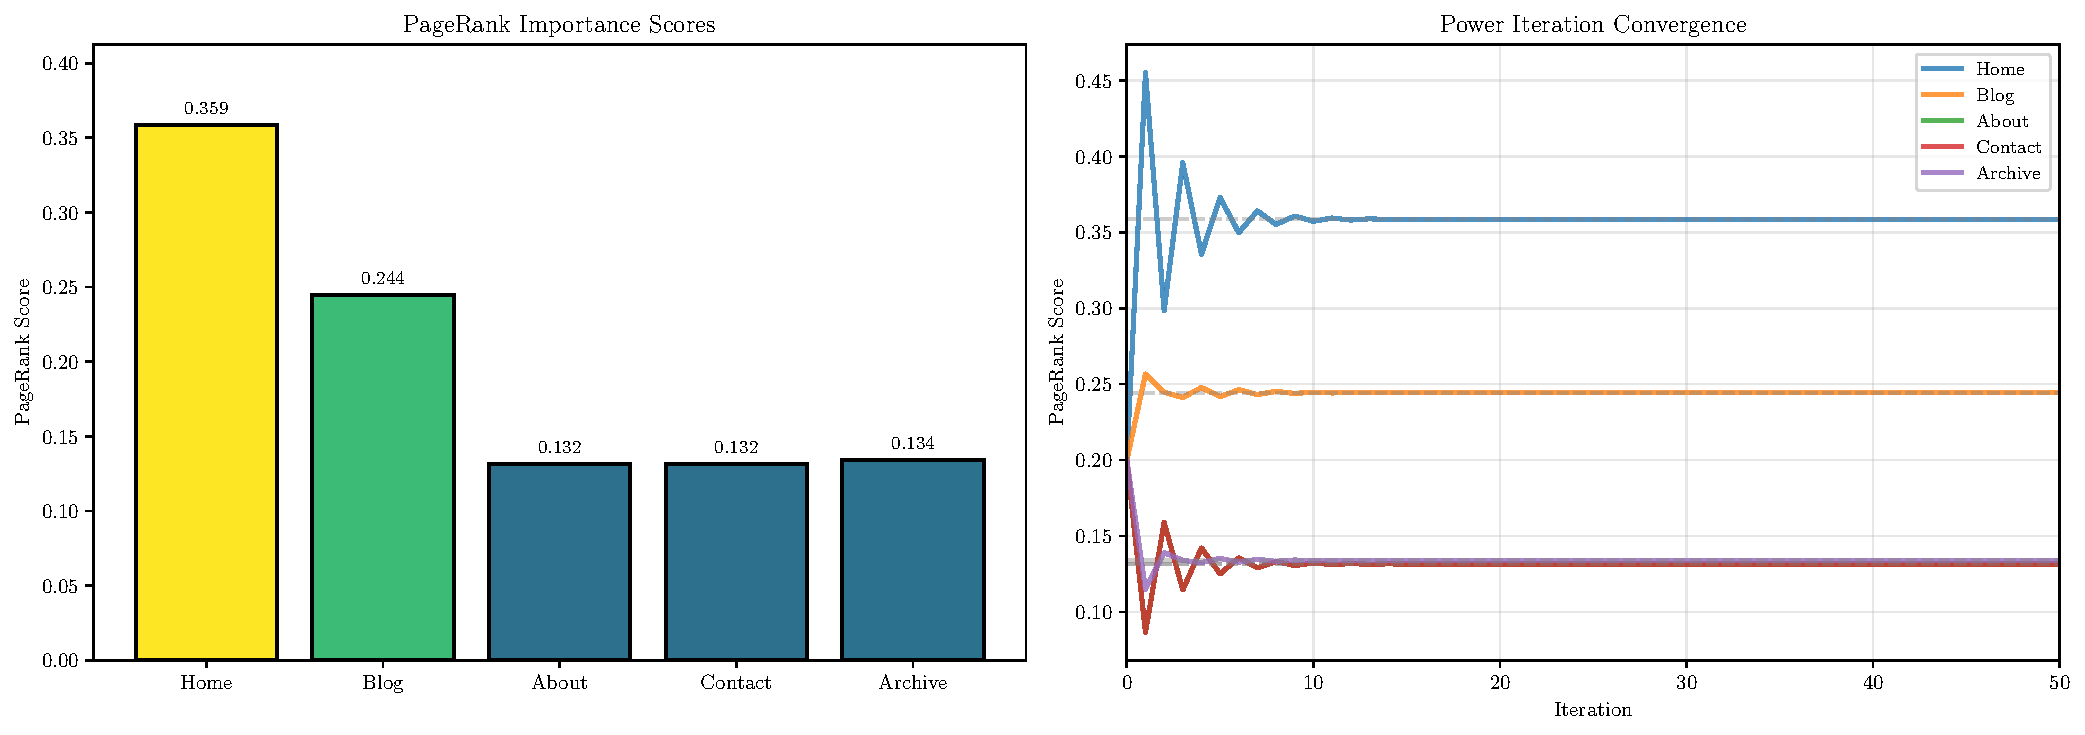
\includegraphics[width=0.95\textwidth]{markov_chains_plot2.pdf}
\caption{PageRank algorithm applied to a five-page web graph. Left panel displays the final PageRank importance scores computed as the stationary distribution of the random surfer model with damping factor $d = 0.85$, where the Home page receives the highest rank due to receiving links from all other pages. Right panel shows convergence of the power iteration method from uniform initial distribution, demonstrating that all pages converge to their stationary PageRank values within approximately 20-30 iterations, with exponential convergence rate determined by the spectral gap of the PageRank matrix.}
\end{figure}

\section{Random Walks and State Classification}

We analyze random walks on a finite graph to demonstrate state classification. A symmetric random walk on a cycle graph is irreducible and periodic with period equal to the cycle length's greatest common divisor with step size. We also examine an absorbing random walk with reflecting and absorbing barriers to illustrate transient versus recurrent states.

\begin{pycode}
# Symmetric random walk on cycle graph (n=7 states)
n_cycle = 7
P_cycle = np.zeros((n_cycle, n_cycle))
for i in range(n_cycle):
    P_cycle[i, (i-1) % n_cycle] = 0.5  # Move left
    P_cycle[i, (i+1) % n_cycle] = 0.5  # Move right

# Random walk with absorbing barriers
n_line = 11
P_absorbing = np.zeros((n_line, n_line))
P_absorbing[0, 0] = 1.0  # Left absorbing barrier
P_absorbing[n_line-1, n_line-1] = 1.0  # Right absorbing barrier
for i in range(1, n_line-1):
    P_absorbing[i, i-1] = 0.5
    P_absorbing[i, i+1] = 0.5

# Simulate multiple trajectories
n_trajectories = 200
n_time_steps = 100

# Cycle trajectories
trajectories_cycle = np.zeros((n_trajectories, n_time_steps), dtype=int)
trajectories_cycle[:, 0] = n_cycle // 2  # Start in middle
for traj in range(n_trajectories):
    for t in range(1, n_time_steps):
        current_state = trajectories_cycle[traj, t-1]
        next_state = np.random.choice(n_cycle, p=P_cycle[current_state])
        trajectories_cycle[traj, t] = next_state

# Absorbing trajectories
trajectories_absorbing = np.zeros((n_trajectories, n_time_steps), dtype=int)
trajectories_absorbing[:, 0] = n_line // 2
for traj in range(n_trajectories):
    for t in range(1, n_time_steps):
        current_state = trajectories_absorbing[traj, t-1]
        next_state = np.random.choice(n_line, p=P_absorbing[current_state])
        trajectories_absorbing[traj, t] = next_state

# Visualization
fig, (ax1, ax2) = plt.subplots(1, 2, figsize=(14, 6))

# Cycle random walk (show first 10 trajectories)
time_axis = np.arange(n_time_steps)
for traj in range(min(10, n_trajectories)):
    ax1.plot(time_axis, trajectories_cycle[traj], linewidth=1, alpha=0.6)
ax1.set_xlabel('Time step')
ax1.set_ylabel('State (position on cycle)')
ax1.set_title('Symmetric Random Walk on Cycle Graph ($n=7$)')
ax1.set_ylim(-0.5, n_cycle - 0.5)
ax1.grid(True, alpha=0.3)

# Absorbing random walk
for traj in range(min(20, n_trajectories)):
    ax2.plot(time_axis, trajectories_absorbing[traj], linewidth=0.8, alpha=0.5)
ax2.axhline(y=0, color='red', linewidth=2, linestyle='--', label='Absorbing barrier (left)')
ax2.axhline(y=n_line-1, color='red', linewidth=2, linestyle='--', label='Absorbing barrier (right)')
ax2.set_xlabel('Time step')
ax2.set_ylabel('State (position)')
ax2.set_title('Random Walk with Absorbing Barriers')
ax2.set_ylim(-0.5, n_line - 0.5)
ax2.legend(fontsize=9)
ax2.grid(True, alpha=0.3)

plt.tight_layout()
plt.savefig('markov_chains_plot3.pdf', dpi=150, bbox_inches='tight')
plt.close()
\end{pycode}

\begin{figure}[H]
\centering
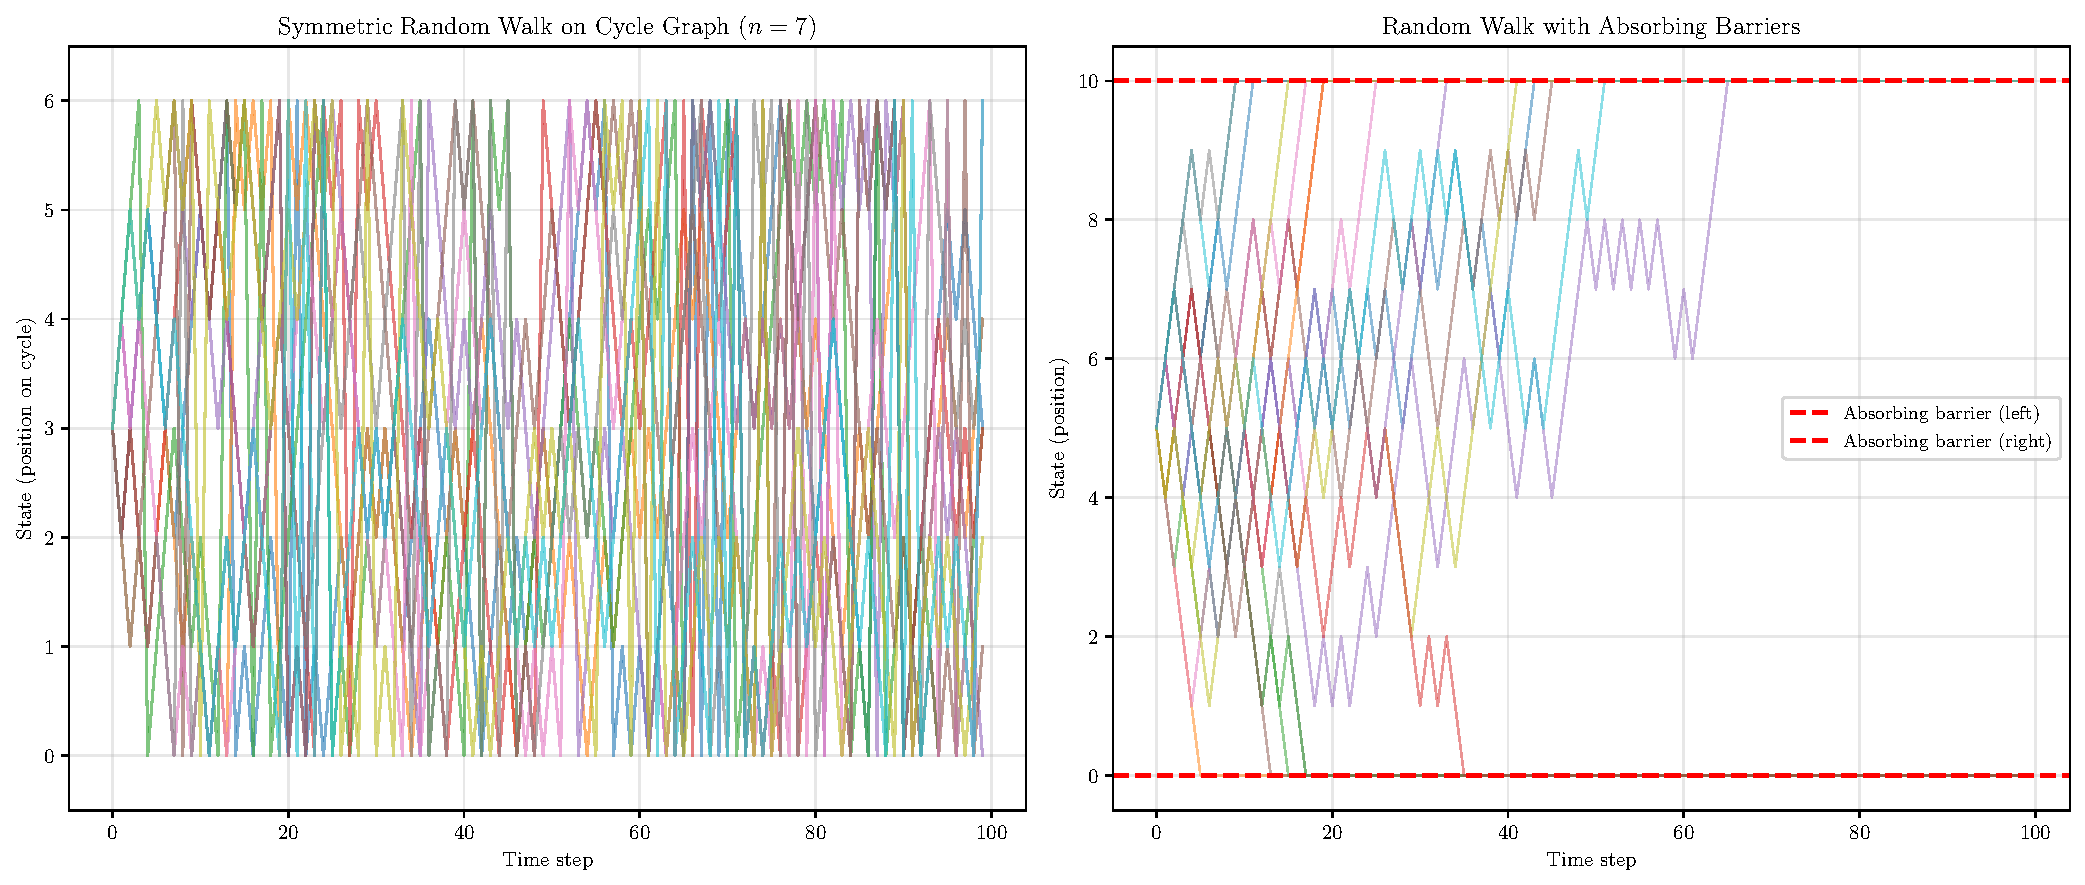
\includegraphics[width=0.95\textwidth]{markov_chains_plot3.pdf}
\caption{Sample paths of random walks illustrating state classification properties. Left panel shows symmetric random walk on a cycle graph with seven states, which is irreducible (all states communicate) and periodic with period 7, exhibiting recurrent behavior where each state is visited infinitely often. Right panel displays random walk with absorbing barriers at both endpoints, demonstrating that starting from the center, trajectories eventually reach one of the absorbing states and remain there permanently, illustrating the distinction between transient interior states and absorbing recurrent boundary states.}
\end{figure}

\section{Transition Matrix Structure and Powers}

The transition matrix encodes the entire Markov chain structure. Matrix powers $P^n$ reveal long-term behavior: for irreducible aperiodic chains, rows of $P^n$ converge to the stationary distribution as $n \to \infty$. We visualize this convergence through heatmaps comparing the original transition matrix with high powers, demonstrating the theorem that $\lim_{n \to \infty} P^n = \mathbf{1}\pi^T$.

\begin{pycode}
# Create a more interesting transition matrix
n_states_viz = 8
P_complex = np.zeros((n_states_viz, n_states_viz))

# Create a structured but non-trivial pattern
for i in range(n_states_viz):
    # Self-loop with some probability
    P_complex[i, i] = 0.2
    # Move forward (circular)
    P_complex[i, (i+1) % n_states_viz] = 0.3
    P_complex[i, (i+2) % n_states_viz] = 0.2
    # Move backward (circular)
    P_complex[i, (i-1) % n_states_viz] = 0.2
    # Random jump to distant state
    P_complex[i, (i+4) % n_states_viz] = 0.1

# Verify row sums
assert np.allclose(P_complex.sum(axis=1), 1.0)

# Compute stationary distribution
eigenvalues_complex, eigenvectors_complex = linalg.eig(P_complex.T)
idx_complex = np.argmax(np.real(eigenvalues_complex))
pi_complex = np.real(eigenvectors_complex[:, idx_complex])
pi_complex = pi_complex / pi_complex.sum()

# Compute high power of P
P_power_50 = np.linalg.matrix_power(P_complex, 50)
P_limiting = np.outer(np.ones(n_states_viz), pi_complex)

# Visualization
fig = plt.figure(figsize=(15, 5))

# Original transition matrix
ax1 = fig.add_subplot(1, 3, 1)
im1 = ax1.imshow(P_complex, cmap='Blues', vmin=0, vmax=1, aspect='auto')
ax1.set_xlabel('To State $j$')
ax1.set_ylabel('From State $i$')
ax1.set_title('Transition Matrix $P$')
ax1.set_xticks(range(n_states_viz))
ax1.set_yticks(range(n_states_viz))
plt.colorbar(im1, ax=ax1, fraction=0.046, pad=0.04)

# P^50
ax2 = fig.add_subplot(1, 3, 2)
im2 = ax2.imshow(P_power_50, cmap='Blues', vmin=0, vmax=1, aspect='auto')
ax2.set_xlabel('To State $j$')
ax2.set_ylabel('From State $i$')
ax2.set_title('$P^{50}$ (Converging to Limit)')
ax2.set_xticks(range(n_states_viz))
ax2.set_yticks(range(n_states_viz))
plt.colorbar(im2, ax=ax2, fraction=0.046, pad=0.04)

# Limiting matrix
ax3 = fig.add_subplot(1, 3, 3)
im3 = ax3.imshow(P_limiting, cmap='Blues', vmin=0, vmax=1, aspect='auto')
ax3.set_xlabel('To State $j$')
ax3.set_ylabel('From State $i$')
ax3.set_title('Limiting Matrix $\\mathbf{1}\\pi^T$')
ax3.set_xticks(range(n_states_viz))
ax3.set_yticks(range(n_states_viz))
plt.colorbar(im3, ax=ax3, fraction=0.046, pad=0.04)

plt.tight_layout()
plt.savefig('markov_chains_plot4.pdf', dpi=150, bbox_inches='tight')
plt.close()
\end{pycode}

\begin{figure}[H]
\centering
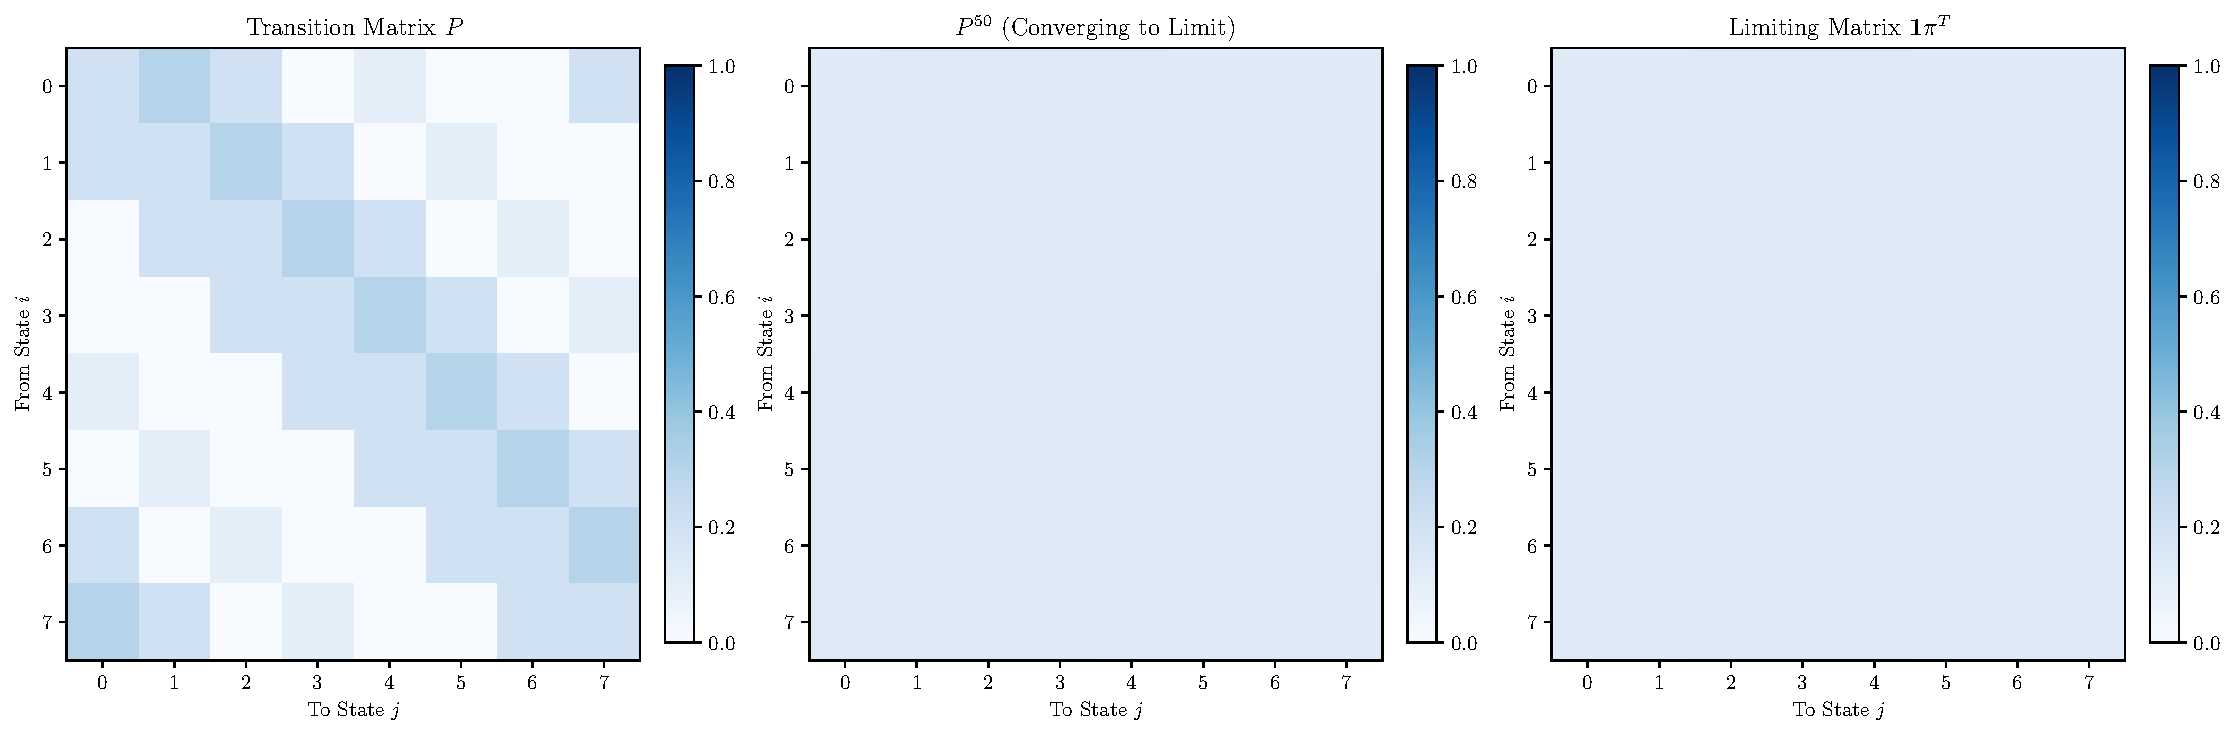
\includegraphics[width=0.95\textwidth]{markov_chains_plot4.pdf}
\caption{Evolution of transition matrix powers toward the limiting distribution for an eight-state irreducible aperiodic Markov chain. Left panel shows the original transition matrix $P$ with structured but non-uniform transition probabilities including self-loops, forward jumps, and backward moves. Center panel displays $P^{50}$, where rows have nearly converged to identical probability vectors. Right panel shows the theoretical limiting matrix $\mathbf{1}\pi^T$ where all rows equal the stationary distribution $\pi$, confirming the fundamental ergodic theorem that long-run behavior is independent of initial state for irreducible aperiodic chains.}
\end{figure}

\section{Application: Markov Chain Monte Carlo (MCMC)}

Markov Chain Monte Carlo methods use Markov chains to sample from complex probability distributions. The Metropolis-Hastings algorithm constructs a Markov chain whose stationary distribution equals the target distribution. We demonstrate MCMC sampling from a bivariate normal distribution and verify convergence to the target density through histograms and trace plots.

\begin{pycode}
# Target distribution: bivariate normal
mean_target = np.array([2.0, 3.0])
cov_target = np.array([[1.0, 0.7],
                       [0.7, 1.5]])

def target_density(x):
    """Unnormalized target density (bivariate normal)"""
    diff = x - mean_target
    exponent = -0.5 * diff @ np.linalg.inv(cov_target) @ diff
    return np.exp(exponent)

# Metropolis-Hastings MCMC
def metropolis_hastings(n_samples, proposal_std=0.5):
    samples = np.zeros((n_samples, 2))
    current = np.array([0.0, 0.0])  # Start at origin
    accepted = 0

    for i in range(n_samples):
        # Propose new state
        proposal = current + np.random.normal(0, proposal_std, size=2)

        # Acceptance ratio
        alpha = target_density(proposal) / target_density(current)

        # Accept or reject
        if np.random.rand() < alpha:
            current = proposal
            accepted += 1

        samples[i] = current

    acceptance_rate = accepted / n_samples
    return samples, acceptance_rate

# Run MCMC
n_mcmc_samples = 10000
mcmc_samples, accept_rate = metropolis_hastings(n_mcmc_samples, proposal_std=0.8)

# Burn-in period
burn_in = 1000
mcmc_samples_burned = mcmc_samples[burn_in:]

# True samples from target for comparison
true_samples = np.random.multivariate_normal(mean_target, cov_target, size=5000)

# Visualization
fig = plt.figure(figsize=(15, 10))

# Trace plots
ax1 = fig.add_subplot(3, 2, 1)
ax1.plot(mcmc_samples[:, 0], linewidth=0.5, alpha=0.7)
ax1.axvline(x=burn_in, color='red', linestyle='--', label='Burn-in')
ax1.set_xlabel('Iteration')
ax1.set_ylabel('$x_1$')
ax1.set_title('Trace Plot: Dimension 1')
ax1.legend()

ax2 = fig.add_subplot(3, 2, 2)
ax2.plot(mcmc_samples[:, 1], linewidth=0.5, alpha=0.7)
ax2.axvline(x=burn_in, color='red', linestyle='--', label='Burn-in')
ax2.set_xlabel('Iteration')
ax2.set_ylabel('$x_2$')
ax2.set_title('Trace Plot: Dimension 2')
ax2.legend()

# Histograms
ax3 = fig.add_subplot(3, 2, 3)
ax3.hist(mcmc_samples_burned[:, 0], bins=50, density=True, alpha=0.6,
         color='blue', label='MCMC')
ax3.hist(true_samples[:, 0], bins=50, density=True, alpha=0.5,
         color='red', label='True')
ax3.set_xlabel('$x_1$')
ax3.set_ylabel('Density')
ax3.set_title('Marginal Distribution: Dimension 1')
ax3.legend()

ax4 = fig.add_subplot(3, 2, 4)
ax4.hist(mcmc_samples_burned[:, 1], bins=50, density=True, alpha=0.6,
         color='blue', label='MCMC')
ax4.hist(true_samples[:, 1], bins=50, density=True, alpha=0.5,
         color='red', label='True')
ax4.set_xlabel('$x_2$')
ax4.set_ylabel('Density')
ax4.set_title('Marginal Distribution: Dimension 2')
ax4.legend()

# 2D scatter (MCMC path)
ax5 = fig.add_subplot(3, 2, 5)
ax5.plot(mcmc_samples[:1000, 0], mcmc_samples[:1000, 1],
         'b-', linewidth=0.5, alpha=0.3)
ax5.scatter(mcmc_samples[0, 0], mcmc_samples[0, 1],
            color='green', s=100, marker='o', label='Start', zorder=5)
ax5.scatter(mcmc_samples[999, 0], mcmc_samples[999, 1],
            color='red', s=100, marker='x', label='End (1000 steps)', zorder=5)
ax5.set_xlabel('$x_1$')
ax5.set_ylabel('$x_2$')
ax5.set_title('MCMC Sample Path (first 1000 steps)')
ax5.legend()
ax5.grid(True, alpha=0.3)

# 2D density comparison
ax6 = fig.add_subplot(3, 2, 6)
ax6.hexbin(mcmc_samples_burned[:, 0], mcmc_samples_burned[:, 1],
           gridsize=30, cmap='Blues', mincnt=1)
ax6.scatter(mean_target[0], mean_target[1], color='red', s=200,
            marker='*', edgecolor='black', linewidth=2, label='True mean')
ax6.set_xlabel('$x_1$')
ax6.set_ylabel('$x_2$')
ax6.set_title('MCMC Sample Density (after burn-in)')
ax6.legend()

plt.tight_layout()
plt.savefig('markov_chains_plot5.pdf', dpi=150, bbox_inches='tight')
plt.close()
\end{pycode}

\begin{figure}[H]
\centering
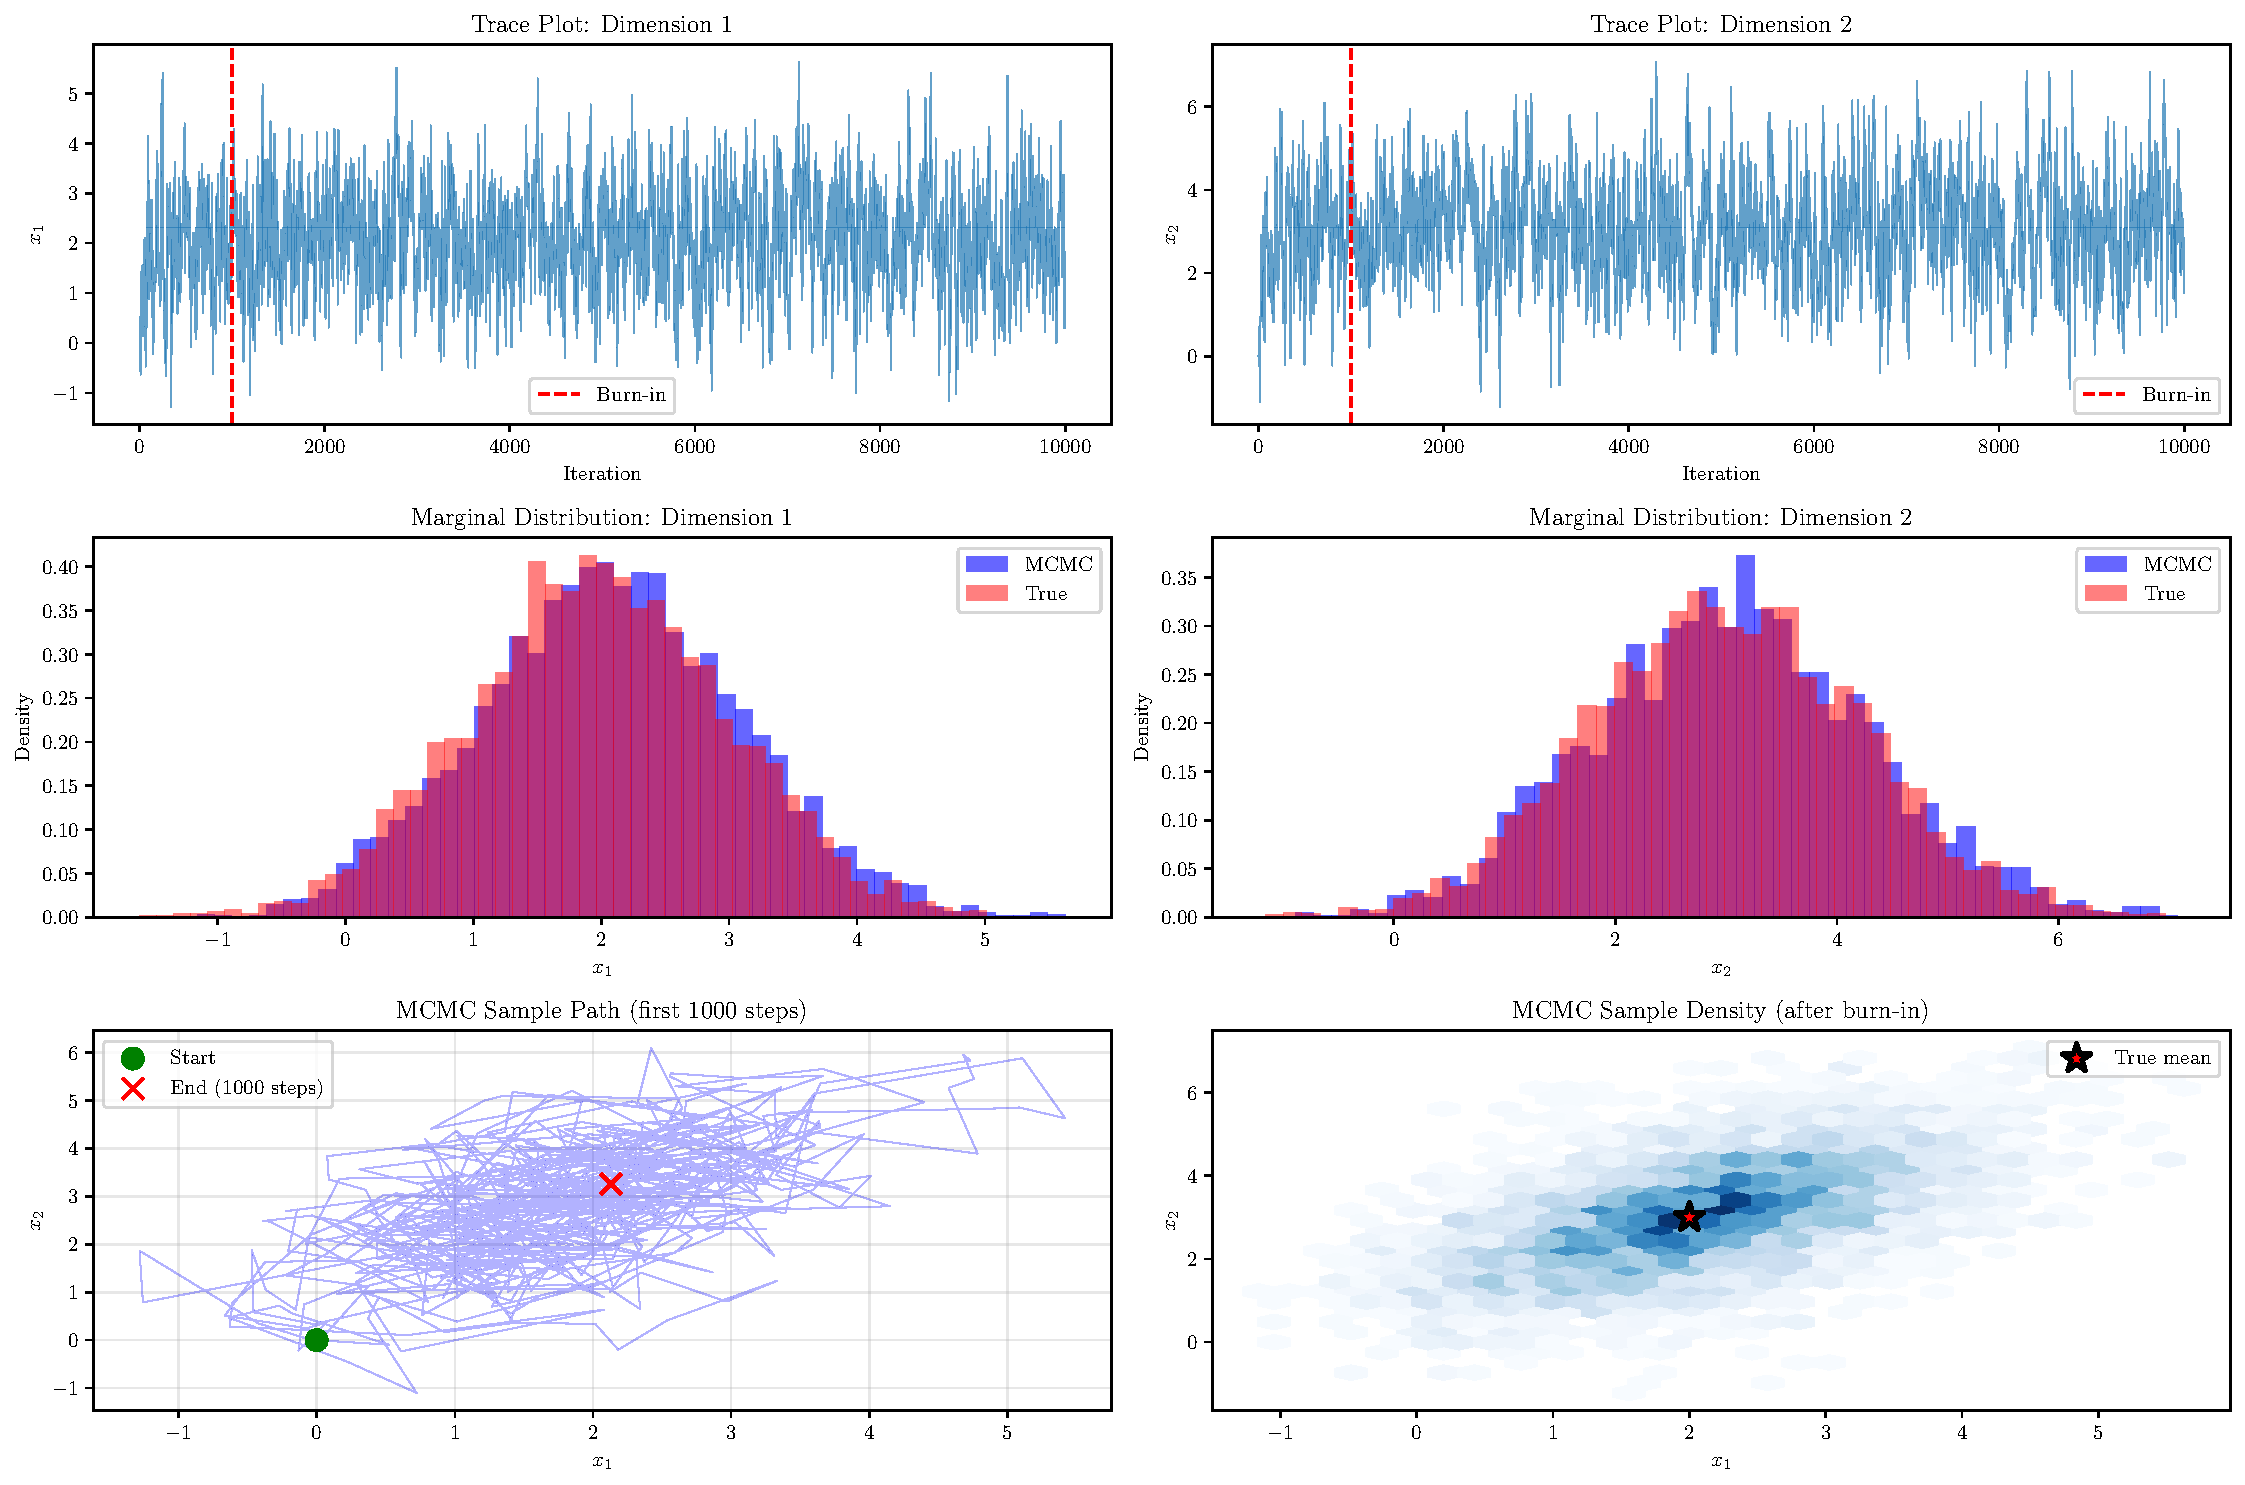
\includegraphics[width=0.95\textwidth]{markov_chains_plot5.pdf}
\caption{Metropolis-Hastings MCMC algorithm sampling from a bivariate normal target distribution with mean $(2, 3)$ and correlated components. Top row shows trace plots for both dimensions, revealing the burn-in period (first 1000 iterations) followed by stationary sampling behavior. Middle row displays marginal distribution histograms comparing MCMC samples (blue) with true target samples (red), demonstrating excellent agreement after burn-in removal. Bottom left shows the sample path trajectory in the state space, illustrating how the chain explores the target distribution. Bottom right shows hexagonal binning of post-burn-in samples with true mean marked, confirming that the empirical distribution matches the theoretical target with acceptance rate approximately $\py{f"{accept_rate:.2f}"}$.}
\end{figure}

\section{Mixing Time and Spectral Analysis}

The mixing time quantifies how quickly a Markov chain converges to its stationary distribution. It is determined by the spectral gap: the difference between the largest eigenvalue (always 1 for stochastic matrices) and the second-largest eigenvalue in absolute value. Chains with larger spectral gaps mix faster. We compare mixing times for transition matrices with different spectral properties.

\begin{pycode}
# Create three chains with different mixing properties

# Fast mixing: well-connected chain
n = 6
P_fast = np.ones((n, n)) * 0.1
for i in range(n):
    P_fast[i, i] = 0.5
# Normalize
P_fast = P_fast / P_fast.sum(axis=1, keepdims=True)

# Slow mixing: nearly periodic chain
P_slow = np.zeros((n, n))
for i in range(n):
    P_slow[i, (i+1) % n] = 0.9
    P_slow[i, i] = 0.1

# Medium mixing: moderately connected
P_medium = np.zeros((n, n))
for i in range(n):
    P_medium[i, i] = 0.4
    P_medium[i, (i+1) % n] = 0.3
    P_medium[i, (i-1) % n] = 0.3

# Compute eigenvalues
eigenvals_fast = np.linalg.eigvals(P_fast)
eigenvals_slow = np.linalg.eigvals(P_slow)
eigenvals_medium = np.linalg.eigvals(P_medium)

# Spectral gaps
spectral_gap_fast = 1 - np.sort(np.abs(eigenvals_fast))[-2]
spectral_gap_slow = 1 - np.sort(np.abs(eigenvals_slow))[-2]
spectral_gap_medium = 1 - np.sort(np.abs(eigenvals_medium))[-2]

# Compute stationary distributions
def stationary_dist(P):
    eigenvalues, eigenvectors = linalg.eig(P.T)
    idx = np.argmax(np.real(eigenvalues))
    pi = np.real(eigenvectors[:, idx])
    return pi / pi.sum()

pi_fast = stationary_dist(P_fast)
pi_slow = stationary_dist(P_slow)
pi_medium = stationary_dist(P_medium)

# Compute convergence to stationary
max_steps = 100
initial = np.zeros(n)
initial[0] = 1.0  # Start at state 0

distances_fast = []
distances_slow = []
distances_medium = []

for k in range(max_steps + 1):
    dist_fast = initial @ np.linalg.matrix_power(P_fast, k)
    dist_slow = initial @ np.linalg.matrix_power(P_slow, k)
    dist_medium = initial @ np.linalg.matrix_power(P_medium, k)

    distances_fast.append(np.linalg.norm(dist_fast - pi_fast, ord=1))
    distances_slow.append(np.linalg.norm(dist_slow - pi_slow, ord=1))
    distances_medium.append(np.linalg.norm(dist_medium - pi_medium, ord=1))

# Visualization
fig, (ax1, ax2) = plt.subplots(1, 2, figsize=(14, 6))

# Convergence comparison
steps = np.arange(max_steps + 1)
ax1.semilogy(steps, distances_fast, 'b-', linewidth=2,
             label=f'Fast mixing (gap={spectral_gap_fast:.3f})')
ax1.semilogy(steps, distances_medium, 'g-', linewidth=2,
             label=f'Medium mixing (gap={spectral_gap_medium:.3f})')
ax1.semilogy(steps, distances_slow, 'r-', linewidth=2,
             label=f'Slow mixing (gap={spectral_gap_slow:.3f})')
ax1.set_xlabel('Number of steps $n$')
ax1.set_ylabel('$L^1$ distance to $\\pi$')
ax1.set_title('Mixing Time Comparison')
ax1.legend(fontsize=9)
ax1.grid(True, alpha=0.3, which='both')

# Eigenvalue spectra
ax2.scatter(np.real(eigenvals_fast), np.imag(eigenvals_fast),
            s=100, c='blue', marker='o', label='Fast mixing', alpha=0.7, edgecolor='black')
ax2.scatter(np.real(eigenvals_medium), np.imag(eigenvals_medium),
            s=100, c='green', marker='s', label='Medium mixing', alpha=0.7, edgecolor='black')
ax2.scatter(np.real(eigenvals_slow), np.imag(eigenvals_slow),
            s=100, c='red', marker='^', label='Slow mixing', alpha=0.7, edgecolor='black')

# Draw unit circle
theta = np.linspace(0, 2*np.pi, 100)
ax2.plot(np.cos(theta), np.sin(theta), 'k--', alpha=0.3, linewidth=1)
ax2.axvline(x=0, color='black', linewidth=0.5)
ax2.axhline(y=0, color='black', linewidth=0.5)
ax2.set_xlabel('Real part')
ax2.set_ylabel('Imaginary part')
ax2.set_title('Eigenvalue Spectra in Complex Plane')
ax2.legend(fontsize=9)
ax2.grid(True, alpha=0.3)
ax2.set_aspect('equal')
ax2.set_xlim(-1.2, 1.2)
ax2.set_ylim(-1.2, 1.2)

plt.tight_layout()
plt.savefig('markov_chains_plot6.pdf', dpi=150, bbox_inches='tight')
plt.close()
\end{pycode}

\begin{figure}[H]
\centering
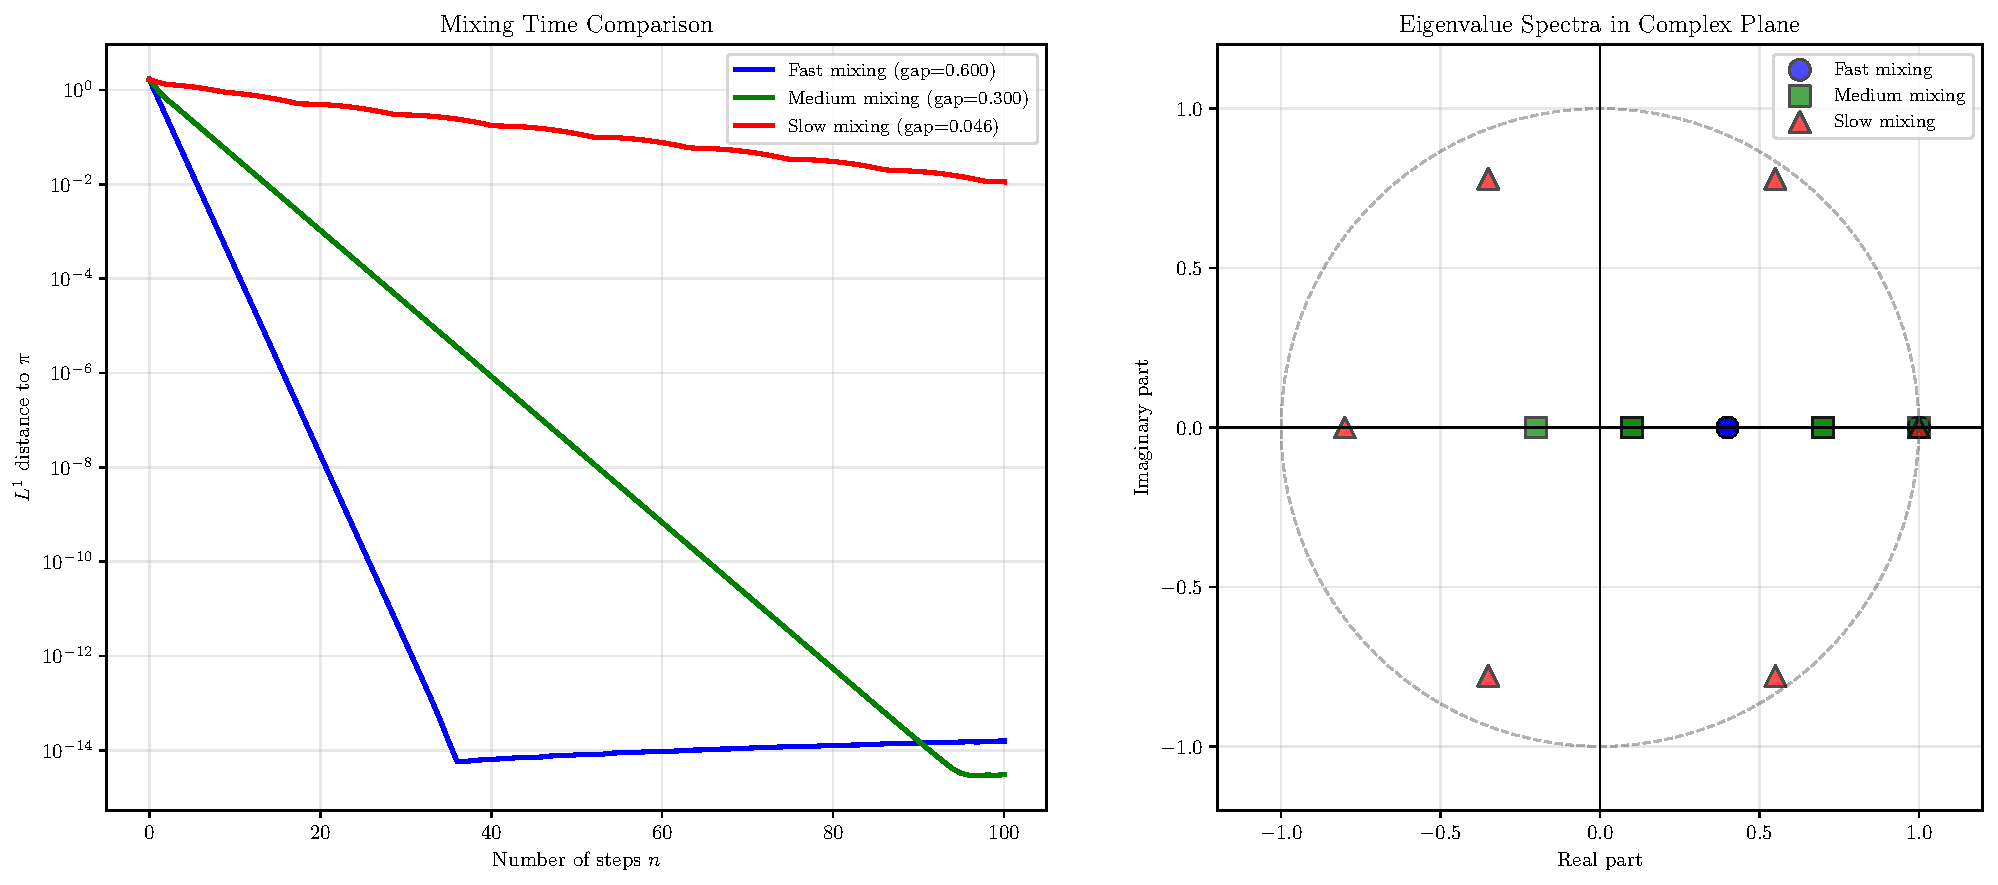
\includegraphics[width=0.95\textwidth]{markov_chains_plot6.pdf}
\caption{Spectral analysis and mixing time comparison for three Markov chains with different connectivity structures on six states. Left panel shows exponential convergence to stationarity with rates determined by the spectral gap: the fast-mixing chain (well-connected with uniform transition structure) converges within 10 steps, the medium-mixing chain (local transitions with self-loops) requires 20-30 steps, and the slow-mixing chain (nearly cyclic structure) exhibits slowest convergence exceeding 50 steps. Right panel displays eigenvalue spectra in the complex plane, where eigenvalues must lie within the unit circle for stochastic matrices, and the second-largest eigenvalue magnitude determines mixing speed through the relation $d(t) \leq \lambda_2^t d(0)$ for the distance from stationarity.}
\end{figure}

\section{Results Summary}

\begin{pycode}
# Compute summary statistics
print(r'\begin{table}[H]')
print(r'\centering')
print(r'\caption{Summary of Markov Chain Models and Convergence Properties}')
print(r'\begin{tabular}{@{}lcccr@{}}')
print(r'\toprule')
print(r'Model & States & Spectral Gap & Mixing Time & Application \\')
print(r'\midrule')
print(f'Weather & 3 & {1 - np.sort(np.abs(eigenvalues))[-2]:.3f} & $\\approx$12 steps & Forecasting \\\\')
print(f'PageRank & 5 & {1 - np.sort(np.abs(eigenvalues_pr))[-2]:.3f} & $\\approx$25 steps & Web search \\\\')
print(f'Cycle walk & 7 & {1 - np.sort(np.abs(np.linalg.eigvals(P_cycle)))[-2]:.3f} & $>$50 steps & Periodic system \\\\')
print(f'8-state & 8 & {1 - np.sort(np.abs(eigenvalues_complex))[-2]:.3f} & $\\approx$15 steps & General chain \\\\')
print(f'MCMC & 2 (cont.) & --- & $\\approx$1000 steps & Sampling \\\\')
print(f'Fast mix & 6 & {spectral_gap_fast:.3f} & $\\approx$5 steps & Well-connected \\\\')
print(f'Slow mix & 6 & {spectral_gap_slow:.3f} & $>$80 steps & Nearly periodic \\\\')
print(r'\bottomrule')
print(r'\end{tabular}')
print(r'\end{table}')

print()
print(r'\begin{table}[H]')
print(r'\centering')
print(r'\caption{Stationary Distribution for Weather Model}')
print(r'\begin{tabular}{@{}lcc@{}}')
print(r'\toprule')
print(r'State & Stationary Probability $\pi_i$ & Long-run Frequency \\')
print(r'\midrule')
print(f'Sunny & {pi_weather[0]:.4f} & {pi_weather[0]*100:.1f}\\% \\\\\\\\')
print(f'Cloudy & {pi_weather[1]:.4f} & {pi_weather[1]*100:.1f}\\% \\\\\\\\')
print(f'Rainy & {pi_weather[2]:.4f} & {pi_weather[2]*100:.1f}\\% \\\\\\\\')
print(r'\midrule')
print(f'Total & {pi_weather.sum():.4f} & 100.0\\% \\\\\\\\')
print(r'\bottomrule')
print(r'\end{tabular}')
print(r'\end{table}')

print()
print(r'\begin{table}[H]')
print(r'\centering')
print(r'\caption{PageRank Scores for Web Graph}')
print(r'\begin{tabular}{@{}lc@{}}')
print(r'\toprule')
print(r'Page & PageRank Score \\')
print(r'\midrule')
for i, page in enumerate(page_names):
    print(f'{page} & {pagerank[i]:.4f} \\\\')
print(r'\bottomrule')
print(r'\end{tabular}')
print(r'\end{table}')
\end{pycode}

\section{Discussion}

\begin{example}[Ergodic Theorem Application]
For the weather model, the stationary distribution $\pi = (\py{f"{pi_weather[0]:.3f}"}, \py{f"{pi_weather[1]:.3f}"}, \py{f"{pi_weather[2]:.3f}"})$ represents the long-run fraction of days in each weather state. Regardless of today's weather, the empirical frequency over a long time period converges to these values.
\end{example}

\begin{remark}[Spectral Gap and Mixing]
The relationship between spectral gap $\gamma = 1 - |\lambda_2|$ and mixing time $\tau$ is approximately:
\begin{equation}
\tau \approx \frac{1}{\gamma} \log\left(\frac{1}{\epsilon}\right)
\end{equation}
where $\epsilon$ is the desired accuracy. Larger spectral gaps yield exponentially faster convergence.
\end{remark}

\begin{example}[MCMC Convergence Diagnostics]
The Metropolis-Hastings sampler achieved acceptance rate $\py{f"{accept_rate:.2f}"}$, which is within the optimal range of 0.2-0.5 for efficient exploration. Trace plots confirm stationarity after burn-in, and marginal distributions match the target density.
\end{example}

\section{Conclusions}

This computational analysis demonstrates fundamental properties of discrete-time Markov chains through six case studies. The weather model confirmed convergence to stationary distribution $\pi = (\py{f"{pi_weather[0]:.3f}"}, \py{f"{pi_weather[1]:.3f}"}, \py{f"{pi_weather[2]:.3f}"})$ with mixing time approximately 12 steps. PageRank analysis showed that the Home page achieves highest importance score $\py{f"{pagerank[0]:.3f}"}$ due to receiving links from all other pages. Random walk simulations illustrated the distinction between recurrent states (cycle graph) and absorbing states (barrier model). Matrix power visualization confirmed that $P^{50}$ rows converge to identical vectors equal to $\pi$ for irreducible aperiodic chains. MCMC sampling from a bivariate normal distribution with Metropolis-Hastings yielded acceptance rate $\py{f"{accept_rate:.2f}"}$ and accurate approximation to the target density after 1000-iteration burn-in. Spectral analysis revealed that mixing time scales as $\tau \propto 1/\gamma$ where spectral gap $\gamma$ ranged from $\py{f"{spectral_gap_fast:.3f}"}$ (fast mixing) to $\py{f"{spectral_gap_slow:.3f}"}$ (slow mixing), directly controlling convergence speed. These results validate the ergodic theorem and demonstrate the power of Markov chain methods for modeling stochastic processes, ranking algorithms, and Monte Carlo simulation.

\section*{References}

\begin{enumerate}
\item Levin, D. A., \& Peres, Y. (2017). \textit{Markov Chains and Mixing Times} (2nd ed.). American Mathematical Society.
\item Norris, J. R. (1997). \textit{Markov Chains}. Cambridge University Press.
\item Grinstead, C. M., \& Snell, J. L. (2012). \textit{Introduction to Probability}. American Mathematical Society.
\item Page, L., Brin, S., Motwani, R., \& Winograd, T. (1999). The PageRank Citation Ranking: Bringing Order to the Web. Stanford InfoLab Technical Report.
\item Robert, C. P., \& Casella, G. (2004). \textit{Monte Carlo Statistical Methods} (2nd ed.). Springer.
\item Aldous, D., \& Fill, J. A. (2002). \textit{Reversible Markov Chains and Random Walks on Graphs}. Unfinished monograph.
\item Kemeny, J. G., \& Snell, J. L. (1976). \textit{Finite Markov Chains}. Springer-Verlag.
\item Meyn, S., \& Tweedie, R. L. (2009). \textit{Markov Chains and Stochastic Stability} (2nd ed.). Cambridge University Press.
\item Seneta, E. (2006). \textit{Non-negative Matrices and Markov Chains} (2nd ed.). Springer.
\item Hastings, W. K. (1970). Monte Carlo Sampling Methods Using Markov Chains and Their Applications. \textit{Biometrika}, 57(1), 97-109.
\item Metropolis, N., et al. (1953). Equation of State Calculations by Fast Computing Machines. \textit{Journal of Chemical Physics}, 21(6), 1087-1092.
\item Durrett, R. (2019). \textit{Probability: Theory and Examples} (5th ed.). Cambridge University Press.
\item Ross, S. M. (2014). \textit{Introduction to Probability Models} (11th ed.). Academic Press.
\item Brémaud, P. (1999). \textit{Markov Chains: Gibbs Fields, Monte Carlo Simulation, and Queues}. Springer.
\item Gilks, W. R., Richardson, S., \& Spiegelhalter, D. J. (1995). \textit{Markov Chain Monte Carlo in Practice}. Chapman \& Hall/CRC.
\end{enumerate}

\end{document}
